% \subsubsection{Comunicação}
\begin{frame}{Divisão de Tarefas no $\mu{}C$}
    \begin{figure}
        \centering
        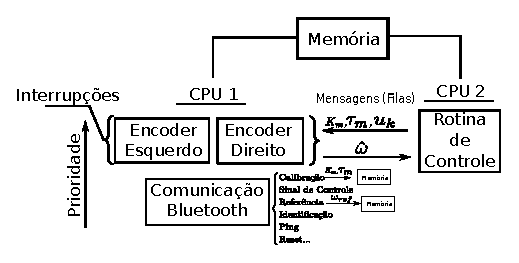
\includegraphics[width=1.0\textwidth]{figuras/ilustracoes/visao_geral_do_sistema.eps}
        \caption{Visão geral do sistema embarcado.}
    \end{figure}
\end{frame}

\begin{frame}{Rotina de Comunicação}
    
    \begin{figure}
        \centering
        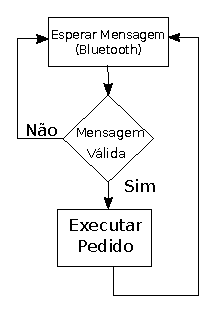
\includegraphics{figuras/ilustracoes/ilustracao_rotina_de_comunicacao.eps}
        \caption{Fluxo grama simplificado da rotina de comunicação.}
    \end{figure}
        
\end{frame}

\begin{frame}{Mensagem}
    \begin{figure}
        \centering
        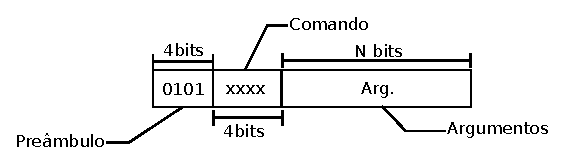
\includegraphics[width=1.0\textwidth]{figuras/ilustracoes/ilustracao_frame_generico.eps}
        \caption{Ilustração de um pacote genérico.}
    \end{figure}
\end{frame}

\begin{frame}{Comandos}
    \begin{align*}
    \text{Comandos}
        \begin{cases}
            \text{Pedir dados da Calibração:} & 0000\\
            \text{Realizar Calibração:} & 0100\\
            \text{Velocidades de Referência:} & 1010\\
            \text{Sinal de Controle:} & 1011\\
            \text{Velocidades Atuais:} & 0011\\
            \text{Iniciar rotina de coleta de dados(\emph{Identify}):} & 0101\\
            \text{Teste de conexão (\emph{Ping}):} & 1111
        \end{cases}
    \end{align*}
\end{frame}

\begin{frame}{Comando:Referência}
    \begin{figure}
        \centering
        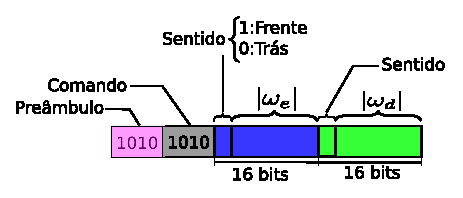
\includegraphics[width=\textwidth]{figuras/ilustracoes/ilustracao_comando_omega_ref.eps}
        \caption{Telecomando de velocidades de referência.}
    \end{figure}
\end{frame}

\begin{frame}{Comando:Sinal de Controle}
    \begin{figure}
        \centering
        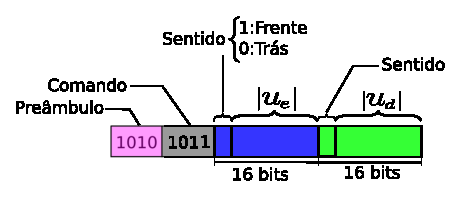
\includegraphics[width=\textwidth]{figuras/ilustracoes/ilustracao_comando_sinal_de_controle.eps}
        \caption{Telecomando de sinal de controle.}
    \end{figure}
\end{frame}

\begin{frame}{Comando:Coleta de Dados}
    \begin{figure}
        \centering
        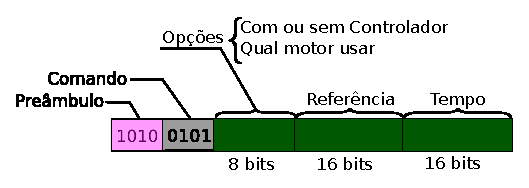
\includegraphics[width=\textwidth]{figuras/ilustracoes/ilustracao_comando_coleta_de_dados.eps}
        \caption{Telecomando para coleta de dados.}
    \end{figure}
\end{frame}